\section{聚类分析}
    \begin{enumerate}
        \item
        {\kaishu \textcolor{blue}{解:}}\\
        {\kaishu \textcolor{blue}{最短距离法:}}
        \begin{enumerate}[label=(\arabic*)]
            \item 聚类过程如下:\\六个样品自成一类$G_k=\{\pmb{x}_i^{\mathrm{T}}\}(k=1,2,\cdots,6)$,先求距离矩阵$\pmb{D}_{(0)}$。
            \begin{table}[H]
                \centering
                \begin{tabular}{|c|c|c|c|c|c|c|}
                    \hline
                    $\pmb{D}_{(0)}$ & $G_1$ & $G_2$ & $G_3$ & $G_4$ & $G_5$ & $G_6$ \\ \hline
                    $G_1$ & $0$ & & & & & \\ \hline
                    $G_2$ & $1$ & $0$ & & & & \\ \hline
                    $G_3$ & $\textit{0.4}$ & $1.4$ & $0$ & & & \\ \hline
                    $G_4$ & $2.5$ & $2.5$ & $2.5$ & $0$ & & \\ \hline
                    $G_5$ & $5.5$ & $6.5$ & $5.1$ & $6$ & $0$ & \\ \hline
                    $G_6$ & $2$ & $3$ & $1.6$ & $2.5$ & $3.5$ & $0$ \\ \hline
                \end{tabular}
            \end{table}
            $\pmb{D}_{(0)}$中最小非零元素为$0.4$,所以将对应的$G_1$和$G_3$合并为新类$G_7=G_1 \cup G_3$,按公式(7.3.2)计算新类$G_7$与其他类的距离,即$D_{7k} = \min\{D_{1k},D_{3k}\}(k= 2,4,5,6)$。其他类与类之间的距离不变,得到距离矩阵$\pmb{D}_{(1)}$。
            \begin{table}[H]
                \centering
                \begin{tabular}{|c|c|c|c|c|c|}
                    \hline
                    $\pmb{D}_{(1)}$ & $G_2$ & $G_4$ & $G_5$ & $G_6$ & $G_7$ \\ \hline
                    $G_2$ & $0$ & & & & \\ \hline
                    $G_4$ & $2.5$ & $0$ & & & \\ \hline
                    $G_5$ & $6.5$ & $6$ & $0$ & & \\ \hline
                    $G_6$ & $3$ & $2.5$ & $3.5$ & $0$ & \\ \hline
                    $G_7$ & $\textit{1}$ & $2.5$ & $5.1$ & $1.6$ & $0$ \\ \hline
                \end{tabular}
            \end{table}
            $\pmb{D}_{(1)}$中最小非零元素为$1$,所以将对应的$G_2$和$G_7$合并为新类$G_8=G_2 \cup G_7$,按公式(7.3.2)计算新类$G_8$与其他类的距离,即$D_{8k} = \min\{D_{2k},D_{7k}\}(k=4,5,6)$。其他类与类之间的距离不变,得到距离矩阵$\pmb{D}_{(2)}$。
            \begin{table}[H]
                \centering
                \begin{tabular}{|c|c|c|c|c|}
                    \hline
                    $\pmb{D}_{(2)}$ & $G_4$ & $G_5$ & $G_6$ & $G_8$ \\ \hline
                    $G_4$ & $0$ & & & \\ \hline
                    $G_5$ & $6$ & $0$ & & \\ \hline
                    $G_6$ & $2.5$ & $3.5$ & $0$ & \\ \hline
                    $G_8$ & $2.5$ & $5.1$ & $\textit{1.6}$ & $0$ \\ \hline
                \end{tabular}
            \end{table}
            $\pmb{D}_{(2)}$中最小非零元素为$1.6$,所以将对应的$G_6$和$G_8$合并为新类$G_9=G_6 \cup G_8$,计算距离矩阵$\pmb{D}_{(3)}$。
            \begin{table}[H]
                \centering
                \begin{tabular}{|c|c|c|c|c|}
                    \hline
                    $\pmb{D}_{(3)}$ & $G_4$ & $G_5$ & $G_9$ \\ \hline
                    $G_4$ & $0$ & & \\ \hline
                    $G_5$ & $6$ & $0$ & \\ \hline
                    $G_9$ & $\textit{2.5}$ & $3.5$ & $0$ \\ \hline
                \end{tabular}
            \end{table}
            $\pmb{D}_{(3)}$中最小非零元素为$2.5$,所以将对应的$G_4$和$G_9$合并为新类$G_{10}=G_4 \cup G_9$,计算距离矩阵$\pmb{D}_{(4)}$。
            \begin{table}[H]
                \centering
                \begin{tabular}{|c|c|c|c|c|}
                    \hline
                    $\pmb{D}_{(4)}$ & $G_5$ & $G_{10}$ \\ \hline
                    $G_5$ & $0$ & \\ \hline
                    $G_{10}$ & $\textit{3.5}$ & $0$ \\ \hline
                \end{tabular}
            \end{table}
            最后,所有样品合并为一,聚类过程结束。
            \item 树形图如下:
            \begin{figure}[H]
                \centering
                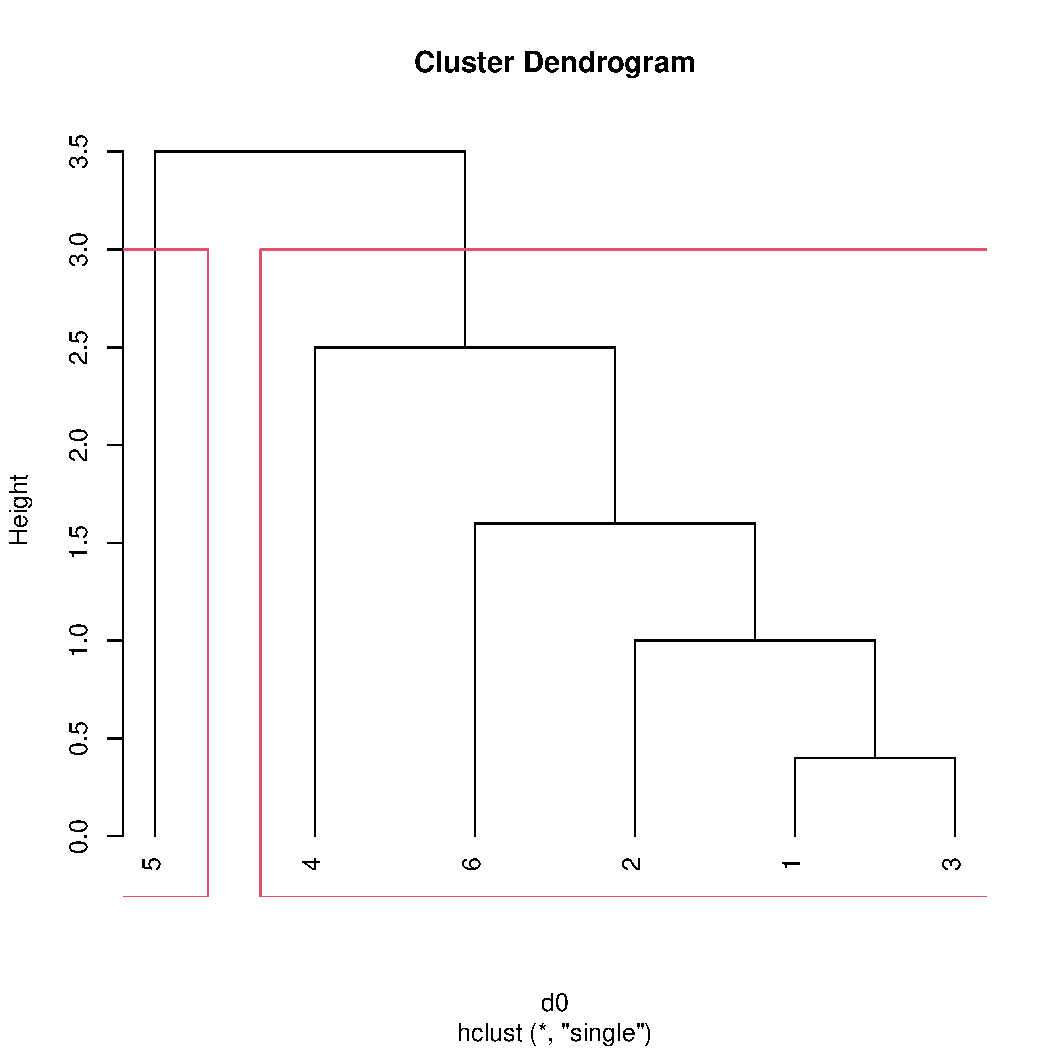
\includegraphics[scale=0.5]{7.1最短距离法.pdf}
                \caption{题1最短距离法树形图}
            \end{figure}
            \item $\pmb{x}_5^{\mathrm{T}}=(\{3,5\})$为一类,其余样品为一类。
        \end{enumerate}
        {\kaishu \textcolor{blue}{最长距离法:}}
        \begin{enumerate}[label=(\arabic*)]
            \item 聚类过程如下:\\
            六个样品自成一类$G_k=\{\pmb{x}_i^{\mathrm{T}}\}(k=1,2,\cdots,6)$,先求距离矩阵$\pmb{D}_{(0)}$。
            \begin{table}[H]
                \centering
                \begin{tabular}{|c|c|c|c|c|c|c|}
                    \hline
                    $\pmb{D}_{(0)}$ & $G_1$ & $G_2$ & $G_3$ & $G_4$ & $G_5$ & $G_6$ \\ \hline
                    $G_1$ & $0$ & & & & & \\ \hline
                    $G_2$ & $1$ & $0$ & & & & \\ \hline
                    $G_3$ & $\textit{0.4}$ & $1.4$ & $0$ & & & \\ \hline
                    $G_4$ & $2.5$ & $2.5$ & $2.5$ & $0$ & & \\ \hline
                    $G_5$ & $5.5$ & $6.5$ & $5.1$ & $6$ & $0$ & \\ \hline
                    $G_6$ & $2$ & $3$ & $1.6$ & $2.5$ & $3.5$ & $0$ \\ \hline
                \end{tabular}
            \end{table}
            $\pmb{D}_{(0)}$中最小非零元素为$0.4$,所以将对应的$G_1$和$G_3$合并为新类$G_7=G_1 \cup G_3$,按公式(7.3.4)计算新类$G_7$与其他类的距离,即$D_{7k} = \max\{D_{1k},D_{3k}\}(k= 2,4,5,6)$。其他类与类之间的距离不变,得到距离矩阵$\pmb{D}_{(1)}$。
            \begin{table}[H]
                \centering
                \begin{tabular}{|c|c|c|c|c|c|}
                    \hline
                    $\pmb{D}_{(1)}$ & $G_2$ & $G_4$ & $G_5$ & $G_6$ & $G_7$ \\ \hline
                    $G_2$ & $0$ & & & & \\ \hline
                    $G_4$ & $2.5$ & $0$ & & & \\ \hline
                    $G_5$ & $6.5$ & $6$ & $0$ & & \\ \hline
                    $G_6$ & $3$ & $2.5$ & $3.5$ & $0$ & \\ \hline
                    $G_7$ & $\textit{1.4}$ & $2.5$ & $5.5$ & $2$ & $0$ \\ \hline
                \end{tabular}
            \end{table}
            $\pmb{D}_{(1)}$中最小非零元素为$1.4$,所以将对应的$G_2$和$G_7$合并为新类$G_8=G_2 \cup G_7$,按公式(7.3.4)计算新类$G_8$与其他类的距离,即$D_{8k} = \max\{D_{2k},D_{7k}\}(k=4,5,6)$。其他类与类之间的距离不变,得到距离矩阵$\pmb{D}_{(2)}$。
            \begin{table}[H]
                \centering
                \begin{tabular}{|c|c|c|c|c|}
                    \hline
                    $\pmb{D}_{(2)}$ & $G_4$ & $G_5$ & $G_6$ & $G_8$ \\ \hline
                    $G_4$ & $0$ & & & \\ \hline
                    $G_5$ & $6$ & $0$ & & \\ \hline
                    $G_6$ & $2.5$ & $3.5$ & $0$ & \\ \hline
                    $G_8$ & $\textit{2.5}$ & $6.5$ & $3$ & $0$ \\ \hline
                \end{tabular}
            \end{table}
            $\pmb{D}_{(2)}$中最小非零元素为$2.5$,所以将对应的$G_4$和$G_8$合并为新类$G_9=G_4 \cup G_8$,计算距离矩阵$\pmb{D}_{(3)}$。
            \begin{table}[H]
                \centering
                \begin{tabular}{|c|c|c|c|c|}
                    \hline
                    $\pmb{D}_{(3)}$ & $G_5$ & $G_6$ & $G_9$ \\ \hline
                    $G_5$ & $0$ & & \\ \hline
                    $G_6$ & $3.5$ & $0$ & \\ \hline
                    $G_9$ & $6.5$ & $\textit{3}$ & $0$ \\ \hline
                \end{tabular}
            \end{table}
            $\pmb{D}_{(3)}$中最小非零元素为$3$,所以将对应的$G_6$和$G_9$合并为新类$G_{10}=G_6 \cup G_9$,计算距离矩阵$\pmb{D}_{(4)}$。
            \begin{table}[H]
                \centering
                \begin{tabular}{|c|c|c|c|c|}
                    \hline
                    $\pmb{D}_{(4)}$ & $G_5$ & $G_{10}$ \\ \hline
                    $G_5$ & $0$ & \\ \hline
                    $G_{10}$ & $\textit{6.5}$ & $0$ \\ \hline
                \end{tabular}
            \end{table}
            最后,所有样品合并为一,聚类过程结束。
            \item 树形图如下:
            \begin{figure}[H]
                \centering
                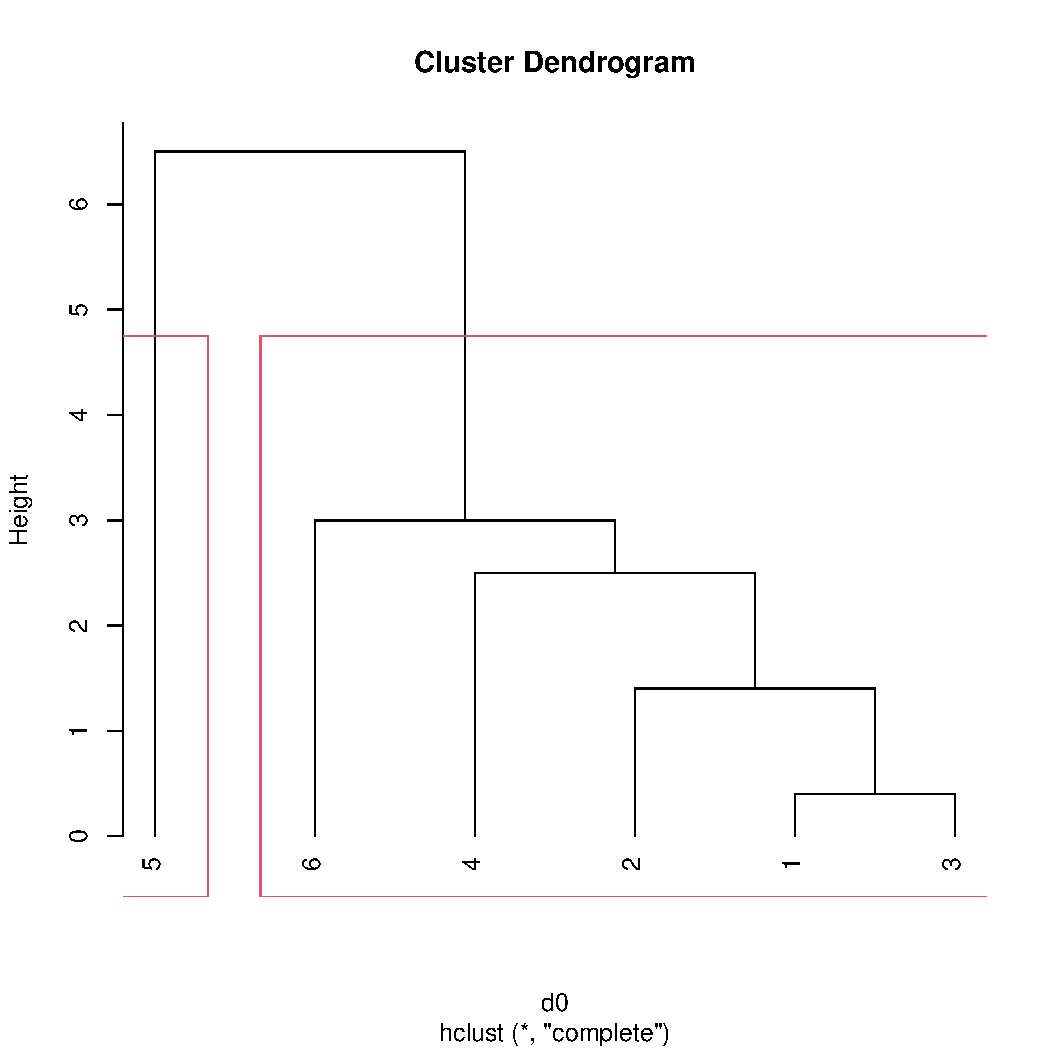
\includegraphics[scale=0.5]{7.1最长距离法.pdf}
                \caption{题1最长距离法树形图}
            \end{figure}
            \item 所以$\pmb{x}_5^{\mathrm{T}}=(\{3,5\})$为一类,其余样品为一类。
        \end{enumerate}
        \code
\begin{lstlisting}
x <- c(1,0.5,1.2,2,3,2.5,1.5,1,1.7,0,5,2.0)
dim(x) <- c(6,2)
d0 <- dist(x, method="minkowski", diag=TRUE, upper=FALSE, p=1)
# 最短距离法
hcs <- hclust(d0, method="single")
plot(hcs, hang=-1)
rect.hclust(hcs, k=2, h=NULL, border=2)
# 最长距离法
hcs <- hclust(d0, method="complete")
plot(hcs, hang=-1)
rect.hclust(hcs, k=2, h=NULL, border=2)
\end{lstlisting}
        \out\\
        输出结果见上。\\
        \summary\\
        主要结论见上。
        \item
        {\kaishu\textcolor{blue}{证:}}
        \begin{align*}
            D_{rk}^2 & =\frac{1}{n_rn_k} \sum\limits_{i \in G_r,j \in G_k}d_{ij}^2\\
            &=\frac{1}{n_rn_k}\left(\sum\limits_{i \in G_p,j \in G_k}d_{ij}^2+\sum\limits_{i \in G_q,j \in G_k}d_{ij}^2\right)\\
            &=\frac{n_p}{n_r} \cdot\frac{1}{n_pn_k} \sum\limits_{i \in G_p,j \in G_k}d_{ij}^2+\frac{n_q}{n_r} \cdot\frac{1}{n_qn_k} \sum\limits_{i \in G_q,j \in G_k}d_{ij}^2\\
            &=\frac{n_p}{n_r}D_{pk}^2+\frac{n_q}{n_r}D_{qk}^2
        \end{align*}
        \item
        {\kaishu \textcolor{blue}{解:}}\\
        {\kaishu \textcolor{blue}{最短距离法:}}
        \begin{enumerate}[label=(\arabic*)]
            \item 聚类过程如下:
            \begin{table}[H]
                \centering
                \begin{tabular}{|c|c|c|c|c|c|c|c|}
                    \hline
                    $\pmb{D}_{(0)}$ & $G_1$ & $G_2$ & $G_3$ & $G_4$ & $G_5$ & $G_6$ & $G_7$\\ \hline
                    $G_1$ & $0$ & & & & & & \\ \hline
                    $G_2$ & $4$ & $0$ & & & & & \\ \hline
                    $G_3$ & $7$ & $3$ & $0$ & & & & \\ \hline
                    $G_4$ & $12$ & $8$ & $5$ & $0$ & & & \\ \hline
                    $G_5$ & $18$ & $14$ & $11$ & $6$ & $0$ & & \\ \hline
                    $G_6$ & $19$ & $15$ & $12$ & $7$ & $\textit{1}$ & $0$ & \\ \hline
                    $G_7$ & $21$ & $17$ & $14$ & $9$ & $3$ & $2$ & $0$ \\ \hline
                \end{tabular}
            \end{table}
            \begin{table}[H]
                \centering
                \begin{tabular}{|c|c|c|c|c|c|c|}
                    \hline
                    $\pmb{D}_{(1)}$ & $G_1$ & $G_2$ & $G_3$ & $G_4$ & $G_7$ & $G_8=G_5 \cup G_6$ \\ \hline
                    $G_1$ & $0$ & & & & & \\ \hline
                    $G_2$ & $4$ & $0$ & & & & \\ \hline
                    $G_3$ & $7$ & $3$ & $0$ & & & \\ \hline
                    $G_4$ & $12$ & $8$ & $5$ & $0$ & & \\ \hline
                    $G_7$ & $21$ & $17$ & $14$ & $9$ & $0$ & \\ \hline
                    $G_8$ & $18$ & $14$ & $11$ & $6$ & $\textit{2}$ & $0$ \\ \hline
                \end{tabular}
            \end{table}
            \begin{table}[H]
                \centering
                \begin{tabular}{|c|c|c|c|c|c|}
                    \hline
                    $\pmb{D}_{(2)}$ & $G_1$ & $G_2$ & $G_3$ & $G_4$ & $G_9=G_7 \cup G_8$ \\ \hline
                    $G_1$ & $0$ & & & & \\ \hline
                    $G_2$ & $4$ & $0$ & & & \\ \hline
                    $G_3$ & $7$ & $\textit{3}$ & $0$ & & \\ \hline
                    $G_4$ & $12$ & $8$ & $5$ & $0$ & \\ \hline
                    $G_9$ & $18$ & $14$ & $11$ & $6$ & $0$ \\ \hline
                \end{tabular}
            \end{table}
            \begin{table}[H]
                \centering
                \begin{tabular}{|c|c|c|c|c|}
                    \hline
                    $\pmb{D}_{(3)}$ & $G_1$ & $G_4$ & $G_9$ & $G_{10}=G_2 \cup G_3$ \\ \hline
                    $G_1$ & $0$ & & & \\ \hline
                    $G_4$ & $12$ & $0$ & & \\ \hline
                    $G_9$ & $18$ & $6$ & $0$ & \\ \hline
                    $G_{10}$ & $\textit{4}$ & $5$ & $11$ & $0$ \\ \hline
                \end{tabular}
            \end{table}
            \begin{table}[H]
                \centering
                \begin{tabular}{|c|c|c|c|c|}
                    \hline
                    $\pmb{D}_{(4)}$ & $G_4$ & $G_9$ & $G_{11}=G_1 \cup G_{10}$ \\ \hline
                    $G_4$ & $0$ & & \\ \hline
                    $G_6$ & $6$ & $0$ & \\ \hline
                    $G_{11}$ & $\textit{5}$ & $11$ & $0$ \\ \hline
                \end{tabular}
            \end{table}
            \begin{table}[H]
                \centering
                \begin{tabular}{|c|c|c|c|c|}
                    \hline
                    $\pmb{D}_{(5)}$ & $G_9$ & $G_{12}=G_4 \cup G_{11}$ \\ \hline
                    $G_9$ & $0$ & \\ \hline
                    $G_{12}$ & $\textit{6}$ & $0$ \\ \hline
                \end{tabular}
            \end{table}
            \item 树形图如下:
            \begin{figure}[H]
                \centering
                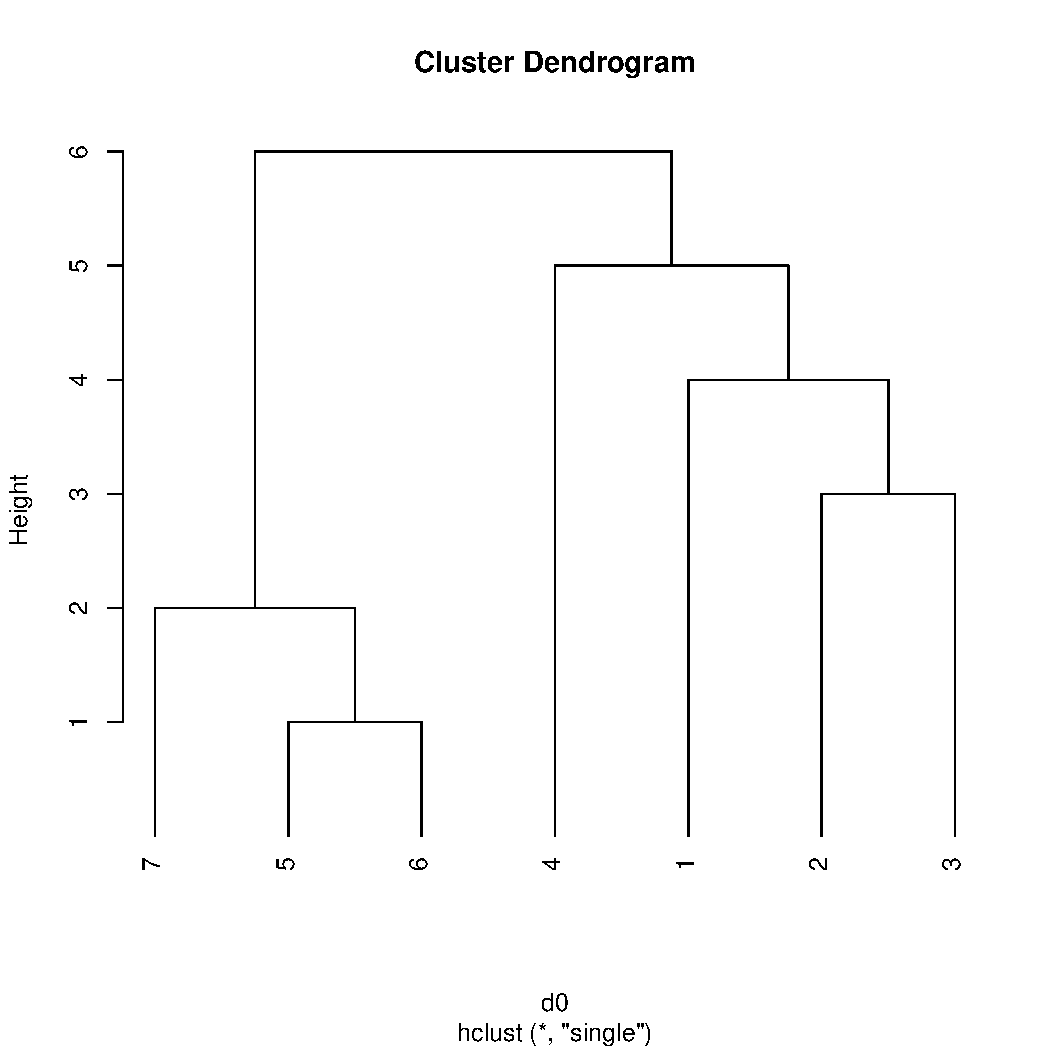
\includegraphics[scale=0.5]{7.3最短距离法.pdf}
                \caption{题3最短距离法树形图}
            \end{figure}
        \end{enumerate}
        {\kaishu \textcolor{blue}{最长距离法:}}
        \begin{enumerate}[label=(\arabic*)]
            \item 聚类过程如下:
            \begin{table}[H]
                \centering
                \begin{tabular}{|c|c|c|c|c|c|c|c|}
                    \hline
                    $\pmb{D}_{(0)}$ & $G_1$ & $G_2$ & $G_3$ & $G_4$ & $G_5$ & $G_6$ & $G_7$\\ \hline
                    $G_1$ & $0$ & & & & & & \\ \hline
                    $G_2$ & $4$ & $0$ & & & & & \\ \hline
                    $G_3$ & $7$ & $3$ & $0$ & & & & \\ \hline
                    $G_4$ & $12$ & $8$ & $5$ & $0$ & & & \\ \hline
                    $G_5$ & $18$ & $14$ & $11$ & $6$ & $0$ & & \\ \hline
                    $G_6$ & $19$ & $15$ & $12$ & $7$ & $\textit{1}$ & $0$ & \\ \hline
                    $G_7$ & $21$ & $17$ & $14$ & $9$ & $3$ & $2$ & $0$ \\ \hline
                \end{tabular}
            \end{table}
            \begin{table}[H]
                \centering
                \begin{tabular}{|c|c|c|c|c|c|c|}
                    \hline
                    $\pmb{D}_{(1)}$ & $G_1$ & $G_2$ & $G_3$ & $G_4$ & $G_7$ & $G_8=G_5 \cup G_6$ \\ \hline
                    $G_1$ & $0$ & & & & & \\ \hline
                    $G_2$ & $4$ & $0$ & & & & \\ \hline
                    $G_3$ & $7$ & $3$ & $0$ & & & \\ \hline
                    $G_4$ & $12$ & $8$ & $5$ & $0$ & & \\ \hline
                    $G_7$ & $21$ & $17$ & $14$ & $9$ & $0$ & \\ \hline
                    $G_8$ & $19$ & $15$ & $12$ & $7$ & $\textit{3}$ & $0$ \\ \hline
                \end{tabular}
            \end{table}
            \begin{table}[H]
                \centering
                \begin{tabular}{|c|c|c|c|c|c|}
                    \hline
                    $\pmb{D}_{(2)}$ & $G_1$ & $G_2$ & $G_3$ & $G_4$ & $G_9=G_7 \cup G_8$ \\ \hline
                    $G_1$ & $0$ & & & & \\ \hline
                    $G_2$ & $4$ & $0$ & & & \\ \hline
                    $G_3$ & $7$ & $\textit{3}$ & $0$ & & \\ \hline
                    $G_4$ & $12$ & $8$ & $5$ & $0$ & \\ \hline
                    $G_9$ & $21$ & $17$ & $14$ & $9$ & $0$ \\ \hline
                \end{tabular}
            \end{table}
            \begin{table}[H]
                \centering
                \begin{tabular}{|c|c|c|c|c|}
                    \hline
                    $\pmb{D}_{(3)}$ & $G_1$ & $G_4$ & $G_9$ & $G_{10}=G_2 \cup G_3$ \\ \hline
                    $G_1$ & $0$ & & & \\ \hline
                    $G_4$ & $12$ & $0$ & & \\ \hline
                    $G_9$ & $21$ & $9$ & $0$ & \\ \hline
                    $G_{10}$ & $\textit{7}$ & $8$ & $17$ & $0$ \\ \hline
                \end{tabular}
            \end{table}
            \begin{table}[H]
                \centering
                \begin{tabular}{|c|c|c|c|c|}
                    \hline
                    $\pmb{D}_{(4)}$ & $G_4$ & $G_9$ & $G_{11}=G_1 \cup G_{10}$ \\ \hline
                    $G_4$ & $0$ & & \\ \hline
                    $G_9$ & $\textit{9}$ & $0$ & \\ \hline
                    $G_{11}$ & $12$ & $21$ & $0$ \\ \hline
                \end{tabular}
            \end{table}
            \begin{table}[H]
                \centering
                \begin{tabular}{|c|c|c|c|c|}
                    \hline
                    $\pmb{D}_{(5)}$ & $G_{11}$ & $G_{12}=G_4 \cup G_9$ \\ \hline
                    $G_{11}$ & $0$ & \\ \hline
                    $G_{12}$ & $\textit{21}$ & $0$ \\ \hline
                \end{tabular}
            \end{table}
            \clearpage
            \item 树形图如下:
            \begin{figure}[H]
                \centering
                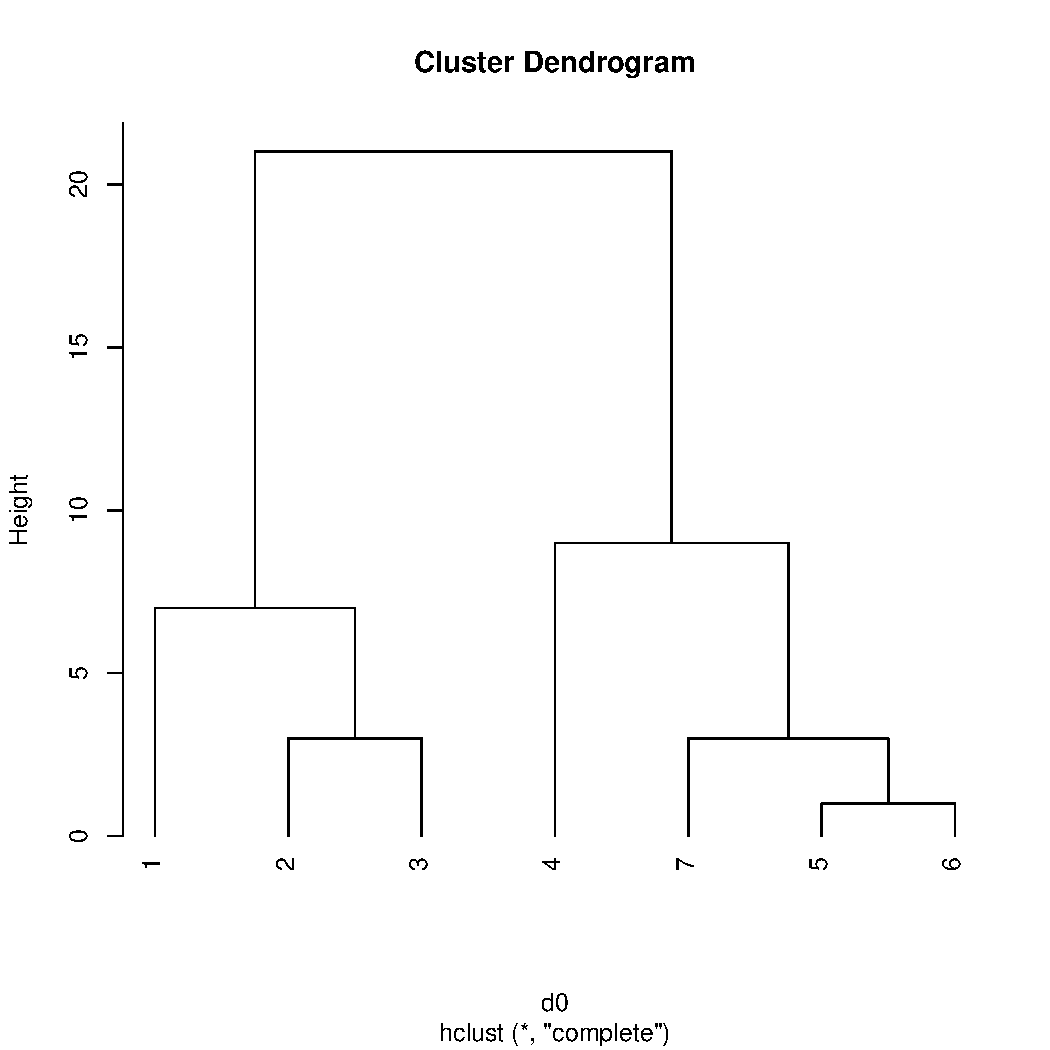
\includegraphics[scale=0.5]{7.3最长距离法.pdf}
                \caption{题3最长距离法树形图}
            \end{figure}
        \end{enumerate}
        \code
\begin{lstlisting}
D <- matrix(c(0,4,7,12,18,19,21,
              0,0,3,8,14,15,17,
              0,0,0,5,11,12,14,
              0,0,0,0,6,7,9,
              0,0,0,0,0,1,3,
              0,0,0,0,0,0,2,
              0,0,0,0,0,0,0), nr=7)
D <- D + t(D)
rownames(D) <- seq(1,7)
d0 <- as.dist(D)
# 最短距离法
hcs <- hclust(d0, method="single")
plot(hcs, hang=-1)
# 最长距离法
hcs <- hclust(d0, method="complete")
plot(hcs, hang=-1)
\end{lstlisting}
        \out\\
        输出结果如上。\\
        \summary\\
        主要结论见上。
        \item
        \code
\begin{lstlisting}
x <- read.table("ex7_4-data.txt", header=TRUE, row.names = 1)
stdx <- scale(x, center=TRUE, scale=TRUE)
# 最短距离法
d0 <- dist(x, method="euclidean", diag=TRUE, upper=FALSE)
hcs <- hclust(d0, method="single")
plot(hcs, hang=-1)
# 最长距离法
d0 <- dist(x, method="euclidean", diag=TRUE, upper=FALSE)
hcs <- hclust(d0, method="complete")
plot(hcs, hang=-1)
# 类平均法,聚为5类
d0 <- dist(x, method="euclidean", diag=TRUE, upper=FALSE)
hcs <- hclust(d0, method="average")
rect.hclust(hcs, k=5, h=NULL, border=2)
plot(hcs, hang=-1)
# 重心法,聚为5类
kmeans(stdx, 5, iter.max=10, algorithm="MacQueen")
\end{lstlisting}
        \out
        \begin{figure}[H]
            \centering
            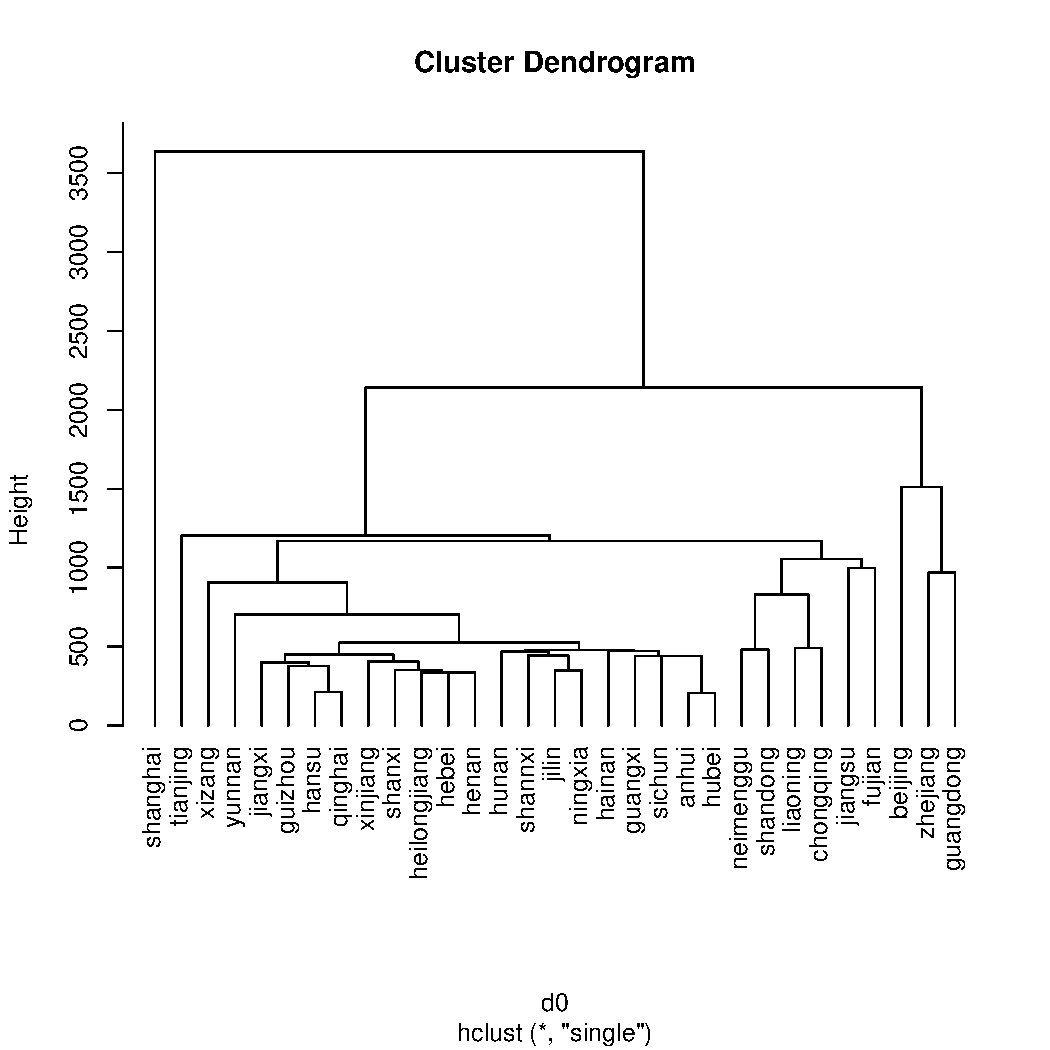
\includegraphics[scale=0.5]{7.4最短距离法.pdf}
            \caption{题4最短距离法树形图}
        \end{figure}
        \begin{figure}[H]
            \centering
            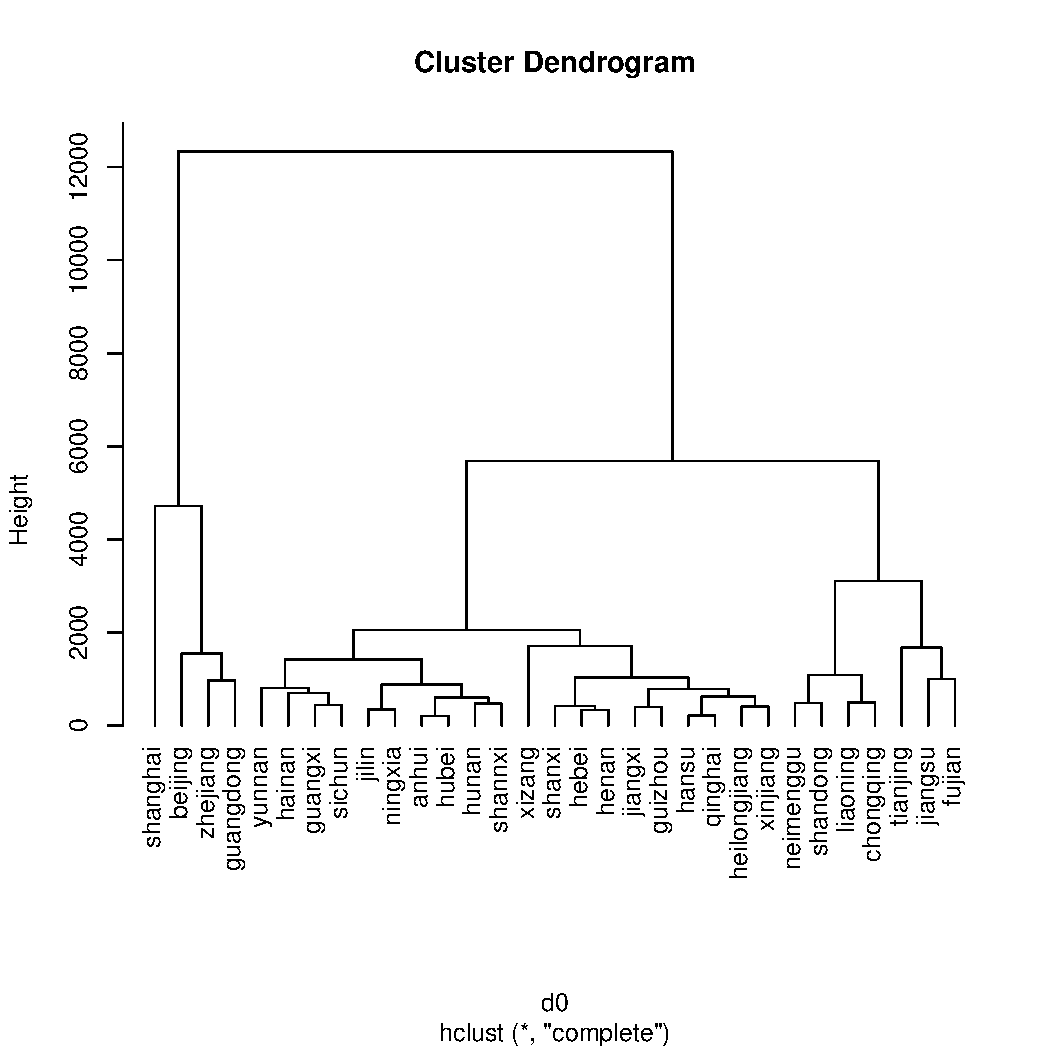
\includegraphics[scale=0.5]{7.4最长距离法.pdf}
            \caption{题4最长距离法树形图}
        \end{figure}
        \begin{figure}[H]
            \centering
            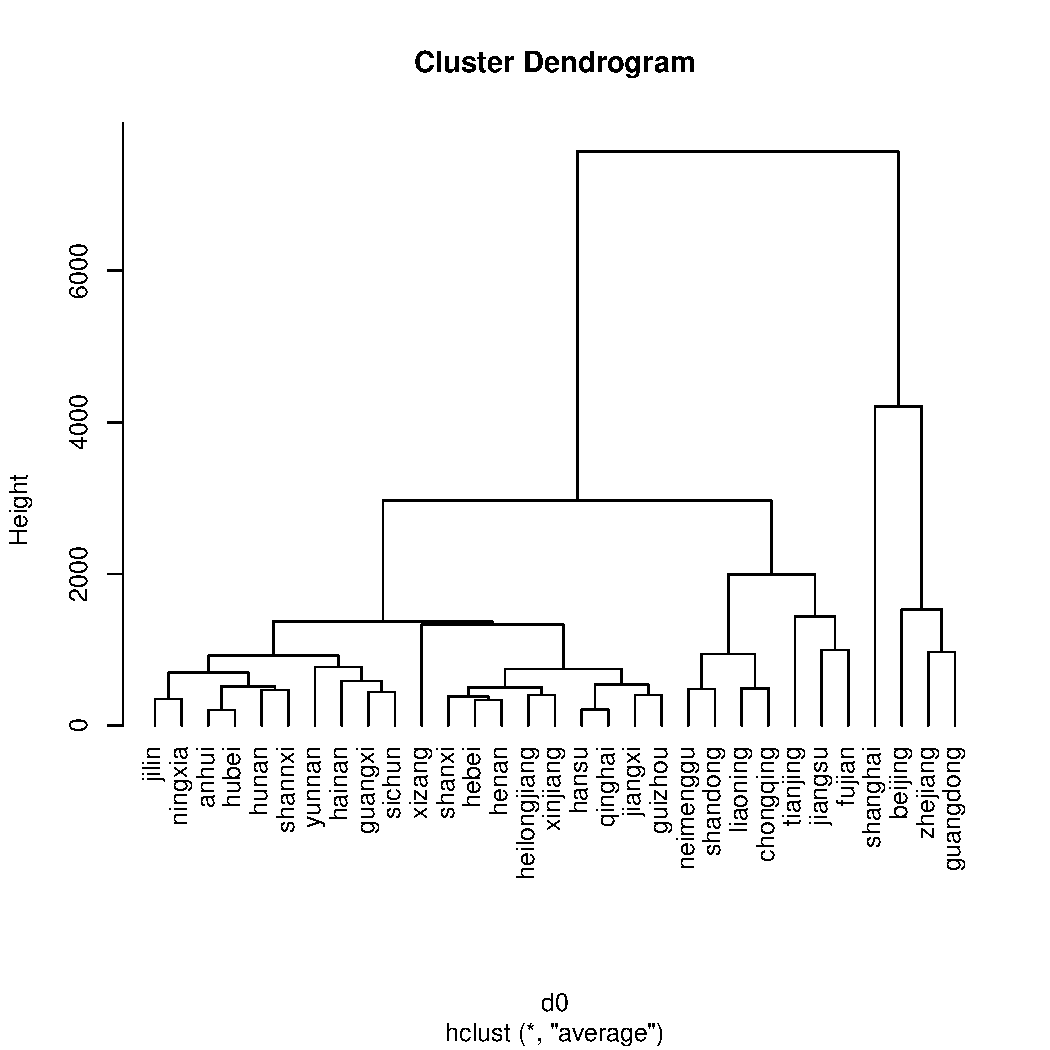
\includegraphics[scale=0.5]{7.4类平均法.pdf}
            \caption{题4类平均法树形图}
        \end{figure}
\begin{lstlisting}
> kmeans(stdx, 5, iter.max=10, algorithm="MacQueen")
K-means clustering with 5 clusters of sizes 10, 5, 3, 11, 2

Cluster means:
     xiaofei     shipin     yizhuo      juzhu jiatingshebei     yiliao   jiaotong
1 -0.4688650 -0.1858709 -0.8724430 -0.5255167   -0.29786714 -0.7981605 -0.3631822
2  1.9568033  1.7878121  0.9215928  1.6390354    1.59656427  1.3068036  1.9033693
3 -0.2694473 -0.5776927  0.2481019  0.7341867   -0.78773623  0.4678536 -0.3847263
4 -0.2592457 -0.5170184  0.3971536 -0.2012223    0.07033978  0.2332705 -0.3693902
5 -0.7176609  0.1699644 -0.4982646 -1.4645628   -1.70733938 -1.2609747 -0.3337768
      jiaoyu
1 -0.4096537
2  1.8461115
3 -0.3023638
4 -0.1503188
5 -1.2867112

Clustering vector:
     beijing     tianjing        hebei       shanxi    neimenggu     liaoning 
           2            2            4            3            4            3 
       jilin heilongjiang     shanghai      jiangsu     zhejiang        anhui 
           3            4            2            4            2            1 
      fujian      jiangxi     shandong        henan        hubei        hunan 
           1            1            4            4            1            4 
   guangdong      guangxi       hainan    chongqing       sichun      guizhou 
           2            1            1            4            1            1 
      yunnan       xizang      shannxi        hansu      qinghai      ningxia 
           5            5            4            1            1            4 
    xinjiang 
           4 

Within cluster sum of squares by cluster:
[1] 18.717017 32.974531  2.251508 19.541294  1.161091
 (between_SS / total_SS =  68.9 %)

Available components:

[1] "cluster"      "centers"      "totss"        "withinss"     "tot.withinss"
[6] "betweenss"    "size"         "iter"         "ifault"
\end{lstlisting}
        \summary\\
        主要结论如上。
        \item
        \code
\begin{lstlisting}
x <- read.table("ex7_5-data.txt", header=TRUE, row.names = 1)
stdx <- scale(x, center=TRUE, scale=TRUE)
set.seed(7)
kmeans(stdx, 5, iter.max=10, algorithm="MacQueen")
\end{lstlisting}
        \out
\begin{lstlisting}
> kmeans(stdx, 5, iter.max=10, algorithm="MacQueen")
K-means clustering with 5 clusters of sizes 11, 7, 4, 2, 7

Cluster means:
        PM10        SO2        CO2     grade2
1  0.1901517  0.2683215  0.6502499 -0.1638951
2 -0.9179291 -0.3624441  0.2052909  1.0339058
3  1.4571533  0.5235103  0.5781826 -1.7822978
4 -1.9628525 -2.1530044 -1.5680164  1.3859312
5  0.3472753  0.2567914 -1.1094977 -0.1538808

Clustering vector:
     Beijing      Tianjin Shijiazhuang      Taiyuan       Hohhot     Shenyang 
           3            1            5            5            2            5 
      Dalian       Harbin     Shanghai      Nanjing     Hangzhou        Hefei 
           2            1            1            1            1            3 
      Fuzhou     Nanchang        Jinan    Zhengzhou        Wuhan     Changsha 
           2            2            5            1            1            1 
   Guangzhou      Nanning       Haikou    Chongqing      Chengdu      Guiyang 
           2            2            4            1            1            5 
     Kunming        Lhasa        Xi'an      Lanzhou       Xining     Yinchuan 
           2            4            1            3            5            5 
      Urumqi 
           3 

Within cluster sum of squares by cluster:
[1]  6.4045158  5.6476870 16.9585359  0.3133693 10.4873904
 (between_SS / total_SS =  66.8 %)

Available components:

[1] "cluster"      "centers"      "totss"        "withinss"     "tot.withinss"
[6] "betweenss"    "size"         "iter"         "ifault"      
\end{lstlisting}
        \summary\\
        为方便固定原始随机点,使用set.seed()播撒随机数种子,根据输出可得到以下分类:
        \begin{enumerate}[label=(\arabic*)]
            \item 第1类(11个):天津、哈尔滨、上海、南京、杭州、郑州、武汉、长沙、重庆、成都、西安;
            \item 第2类(6个):呼和浩特、福州、南昌、广州、南京、昆明;
            \item 第3类(3个):北京、兰州、乌鲁木齐;
            \item 第4类(2个):海口、拉萨;
            \item 第5类(7个):石家庄、太原、沈阳、济南、贵阳、西宁、银川。
        \end{enumerate}
    \end{enumerate}
\clearpage